%\documentclass[10pt,a4paper]{report}
\documentclass[pdf]{beamer}
\usepackage[utf8]{inputenc}
\usepackage{amsmath}
\usepackage{amsfonts}
\usepackage{amssymb}
\usepackage{graphicx}
\usepackage{caption}
\usepackage{subcaption}
\mode<presentation>{}
%%preamble
\title{Pattern recognition and drone controlling with OpenCV}
\author{Gabriel Hidasy, HIRWAAT.PTE, University of Pécs, CsF - CAPES}
\begin{document}

\begin{frame}
\titlepage
\end{frame}
\begin{frame}
	This project aims to produce a framework for controlling the drone from
a computer and integrate it with a pattern recognition algorithm to follow the
pattern in a room.
\end{frame}
\begin{frame}
	A Parrot AR Drone 2.0 was used in the project.
\begin{figure}[hbtp]
  \centering
\begin{subfigure}{.99\textwidth}
  \centering
  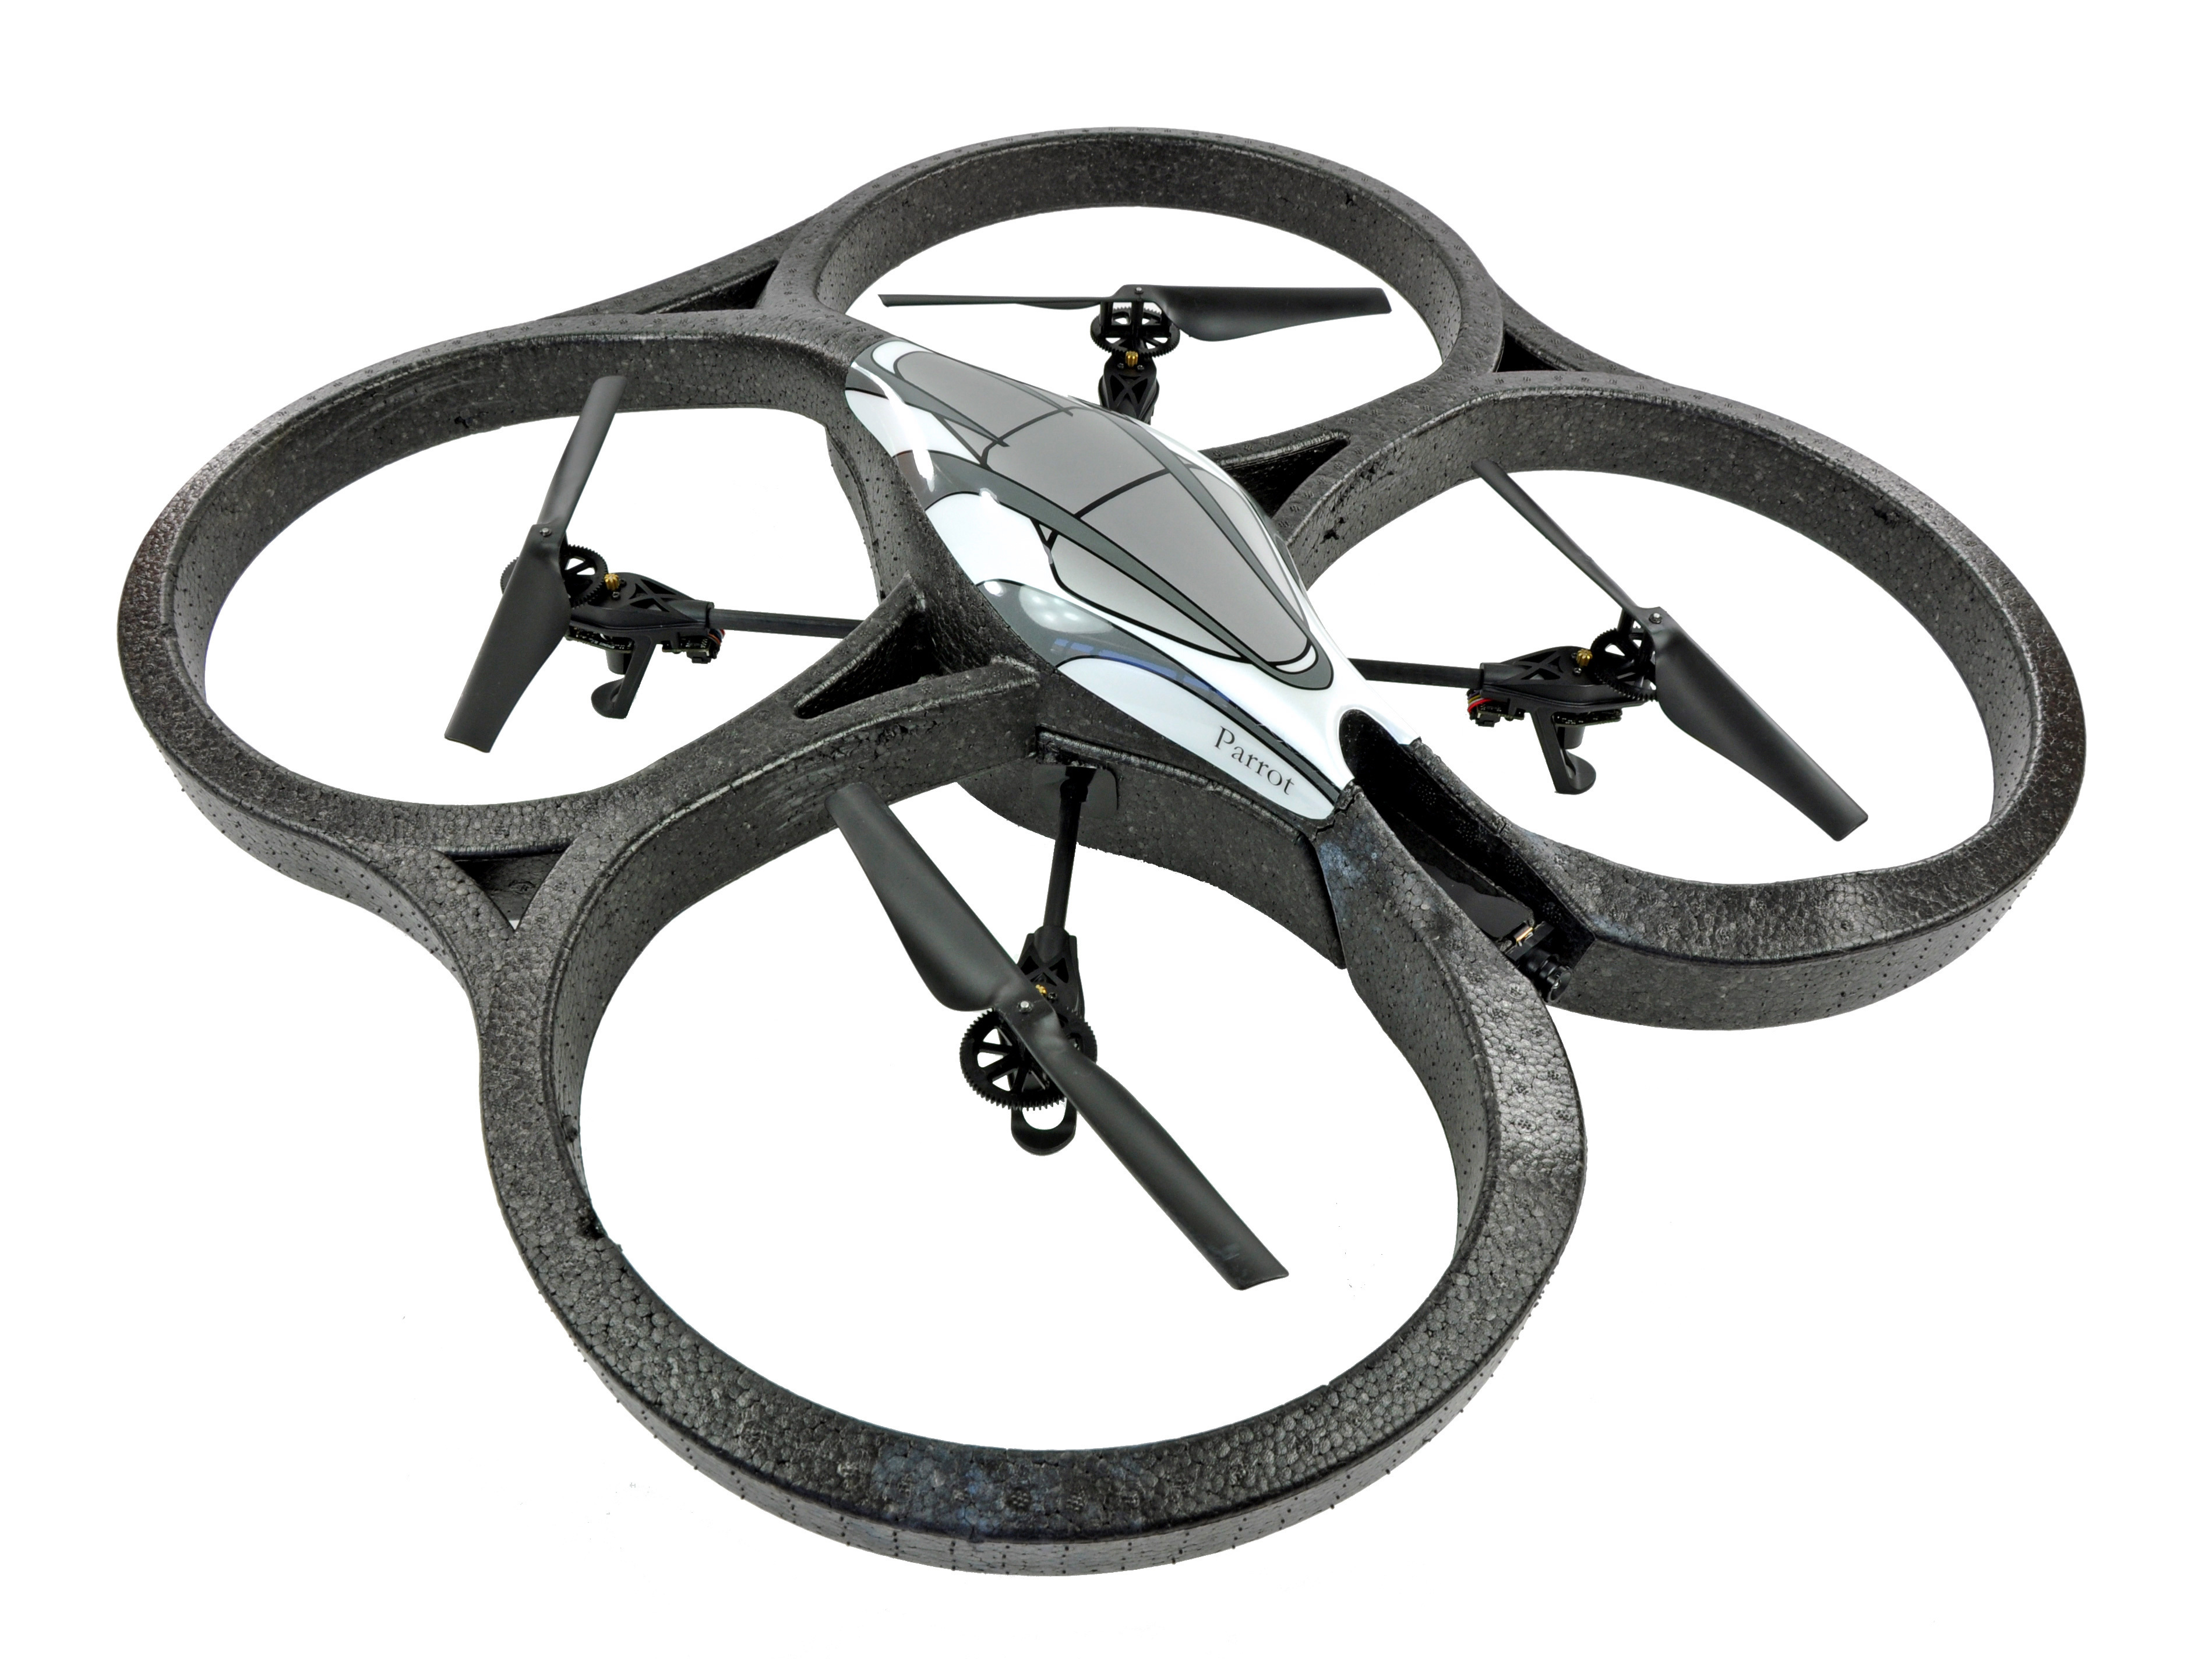
\includegraphics[width=.8\linewidth]{drone.jpg}
\end{subfigure}
\end{figure}
\end{frame}

\begin{frame}
Pattern matching can be done using a combination of two popular algorithms, SURF
for extracting robust features from an image, and FLANN for finding matches.
\end{frame}

\begin{frame}
\begin{figure}[hbtp]
  \centering
SURF\\
\begin{subfigure}{0.80\textwidth}
  \centering
  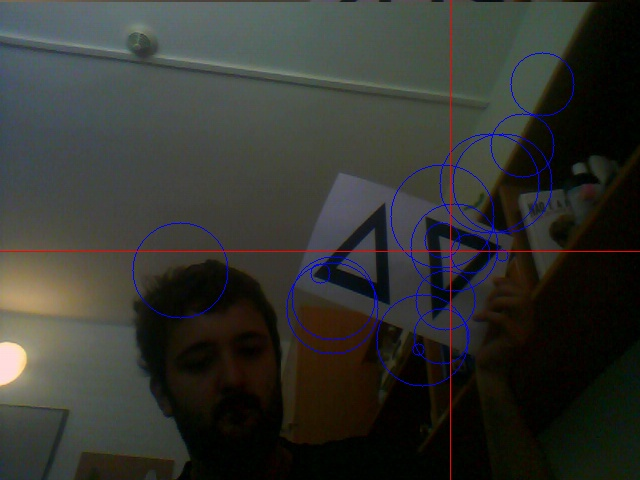
\includegraphics[width=1.0\linewidth]{image_marked.jpg}\\
  The size of the circle indicates the confidence in the match, this circles are
already filtered.
\end{subfigure}
\end{figure}
\end{frame}

\begin{frame}
\begin{figure}[hbtp]
  \centering
FLANN
\begin{subfigure}{1.00\textwidth}
  \centering
  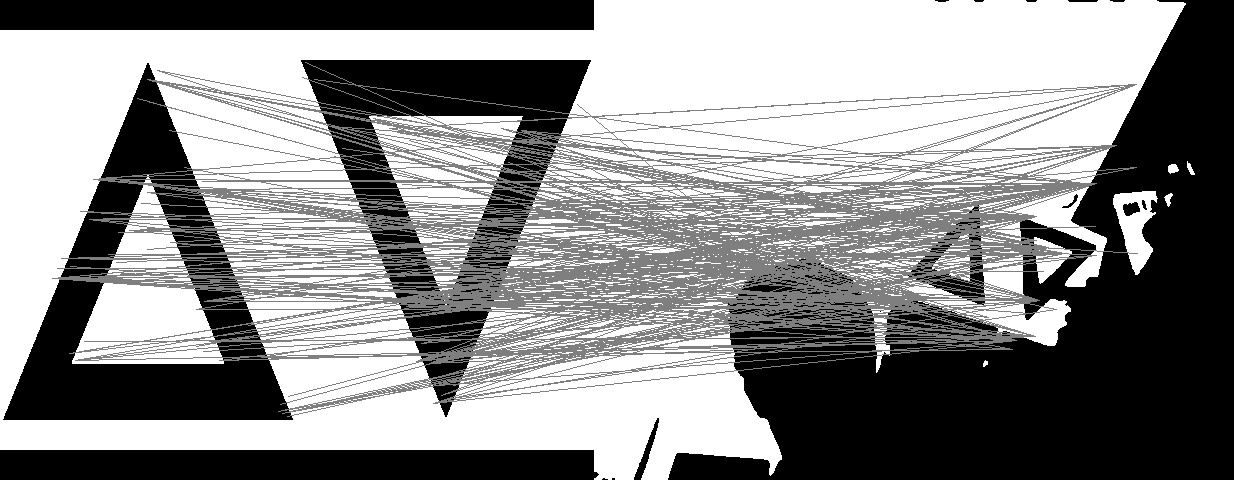
\includegraphics[width=1.00\linewidth]{matches.jpg}\\
The lines demonstrate matches between points in the template and points in the
detected image
\end{subfigure}
\end{figure}
\end{frame}
\begin{frame}
Its possible to see in the previous image the majority of the points detected
are trully part of the template, this is further filtered resulting in a good
acuracy.\\
A decision algorithm was made to command the drone based on the position and
size of the detected pattern.
\end{frame}
\end{document}
